
\documentclass[12pt]{article} 
\usepackage[utf8]{inputenc}
\usepackage[slovak]{babel}
\usepackage[hidelinks,unicode = true]{hyperref}
\usepackage{outline}
\usepackage{graphicx}
%\usepackage{biblatex}
%\addbibresource{literatura.bib}
\usepackage{cite}
\usepackage{caption}
\setcounter{secnumdepth}{3}
\setcounter{tocdepth}{3}

%===========================================================================
\begin{document}           % Konec preambule a zároveň začátek vlastního textu
\begin{titlepage}
\centering
\Large \textbf{České vysoké učení technické v Praze }\\ Fakulta stavební
\vspace{2cm}

\begin{figure}[h!] %logoCVUT
\centering
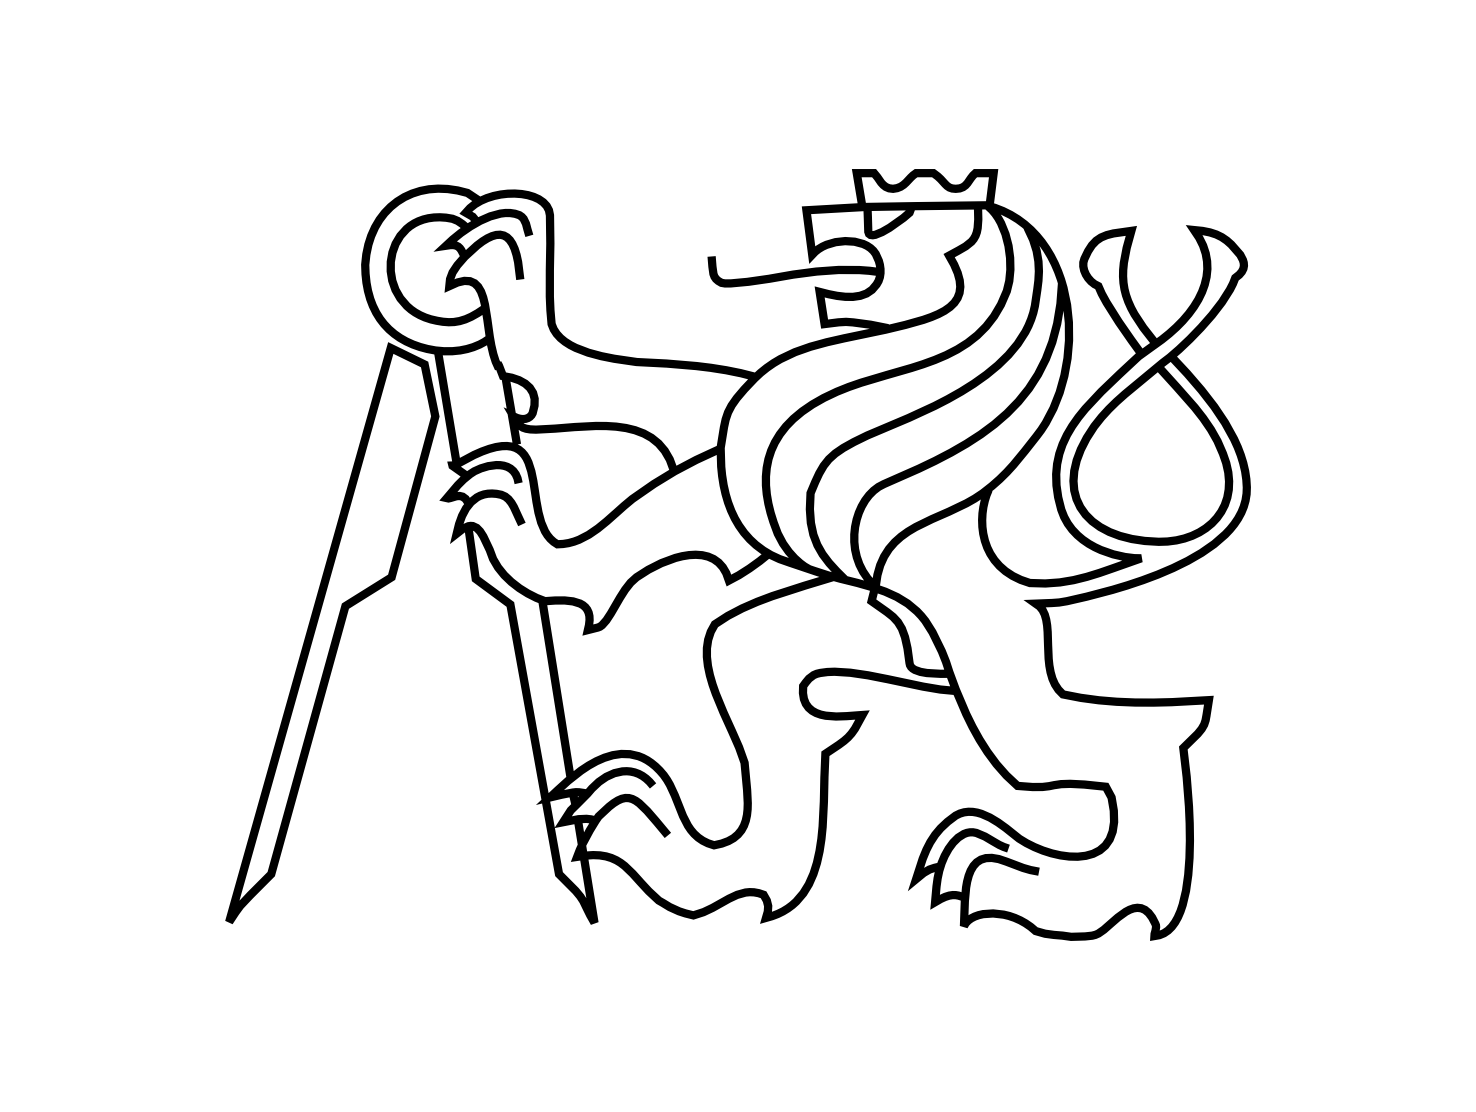
\includegraphics[width=7cm]{./img/cvut.png}
\end{figure}
 
\Large \textbf{155ADKG Algoritmy v digitální kartografii}
\vspace{1cm}

\LARGE  \textbf{ Konvexné obálky a ich konštrukcie}
\vspace{3cm}

\Large Bc. Lukáš Kettner Bc. Martin Hulín \\ 5.11.2019

 \thispagestyle{empty} %neočísluje první stránku
\end{titlepage}

\tableofcontents    % vytváří  Obsah 
\newpage %začne na nové stránce
%------------------------------------------------------------------------
\section{Zadanie}
Vytvorte aplikáciu s grafickým rozhraním, ktorá vygeneruje konvexnú obálku podľa zvoleného typu algoritmu. Vstup do aplikácie : množina bodov  \{p1, …, pn\} . Výstup aplikácie : konvexná obálka  \textit{H}(P).

Nad množinou   \textit{P} implementujte nasledujúce algoritmy pre konštrukciu \textit{H}(P).

\begin{itemize}
\item Jarvis Scan
\item Quick Hull
\item Sweep Line
\end{itemize}
		
Vstupné množiny vrátane vygenerovaných konvexných obálok vhodne vizualizujte. Vytvorte grafy pre množiny n $\in$ $\langle$ 1000, 1000 000 $\rangle$ ilustrujúce doby behu algoritmu. Meranie prevádzajte pre rôzne typy množín opakovane 10x a uvedťe rozptyl. Namerané údaje usporiadajte do tabuliek.

Taktiež sa zamyslite nad problémom singularít pre rôzne typy vstupných množín a nad možnými optimalizáciami. Zhodnoťte dosiahnuté výsledky. Rozhodnite, ktorá z týchto metód je vzhľadom na časovú náročnosť a typ vstupnej množiny najvhodnejšia.

\subsection{Bonusové úlohy}
V rámci úlohy sú vypracované tieto bonusové úlohy

\begin{itemize}
\item Konštrukcia konvexnej obálky metódou Graham Scan.
\item Ošetrenie singulárneho prípadu pro Jarvis Scan
\item Algoritmus pre automatické generovanie konvexných / nekonvexných množín
\end{itemize}
%------------------------------------------------------------------------
\clearpage 
\section{Popis a rozbor problému}
Konvexná obálka je skupina bodov, ktorých spojením vznikne ohraničenie pre všetky ostatné body množiny. Pre konvexnú obálku platí : 

\begin{itemize}
\item žiadny bod vstupnej množiny \textit{P} neleží mimo ohraničenia konvexnej obálky.
\item všetky spojnice bodovvstupnej množiny \textit{P} ležia vnútri konvexnej obálky alebo tvoria jej ohraničenie.
\item všetky vnútorné uhly medzi susednými segmentami konvexnej pbálky sú menšie ako 180 stupňov.
\end{itemize}

\begin{center}
   \includegraphics[width=12cm]{./img/ch_obrazok1.png}
   \captionof{figure}{Princíp konvexnej obálky}
\end{center}

Konvexnú obálku je možné zostrojiť viacerými metódami. V rámci našej práce sme zostrojili algoritmus Jarvis Scan, Quick Hull, Sweep Line a Graham scan.

%------------------------------------------------------------------------
\clearpage 
\section {Popis použitých algoritmov}
\subsection {Jarvis Scan}
Tento algoritmus predstavuje jeden z najpoužívanejích postupov pre tvorbu konvexnej obálky. V algoritme sa zavádza kritérium maximálneho uhlu ($\omega_{max}$). Pri tomto kritériu posudzujeme uhol medzi poslednou stranou konvexnej obálky a úsečkou posledný bod obálky - aktuálny bod. Kritérium hladá taký aktuálny bod, pre ktorý je uhol ($\omega$) maximálny. 
Postup je nasledovný. V prvom kroku vyberieme pivot q so súradnicou $y_{min}$, tento bod je automaticky súčasťou konvexnej obálky. Zavádzame kritérium maximálneho uhlu ($\omega_{max}$). Keď nájdeme bod odpovedajúci kritériu, prídáme takýto bod do konvexnej obálky. Algoritmus končí v momente keď sa dostaneme opäť k pivotu q. 

\subsubsection {Implementácia metódy}
\begin{enumerate}
\item Nájdi pivot q. Zoraď body podľa súradnice y. $ q : y_{min}$
\item Do konvexnej obálky pridaj $q$
\item Inicializuj  $p_{j-1} \in X, p_j = q, p_{j+1} = p_{j-1}$
\item Opakuj pokial $p_{j+1} != q$
\item \hspace {1.5cm} Nájdenie bodu pre ktorý je uhol omega maximálny $p_{j+1} = argmax_{pi \in P} \angle(p_{j-1}, p_j, p_i)$
\item \hspace {1.5cm} Pridaj nájdený bod  $p_{j+1}$ do konvexnej obálky
\item \hspace {1.5cm} Inicializuj $p_{j-1} = p_j , p_j = p_{j+1}$ 
\end{enumerate}

\subsubsection {Problematické situácie}
Problematickou situáciou sú vyskytujúce sa kolineárne body. V takomto prípade je potrebné ošetriť aby sa do konvexnej obálky dostal najvzdialenejší bod.

\subsection {Quick Hull}
Tento algoritmus uplatňuje pri konštrukcii konvexnej obálky princím rozdeľuj a panuj. Jedná sa rekurzívny algoritmus. Skladá sa z lokálnej a globálnej procedúry. Konvexná obálke je skonštruovaná z dvoch častí - upper hull a lower hull. Deliacou priamkou je spojnica dvoch bodov s extrémnymi súradnicami x (minimum, maximum). S oboma časťami obálky sa počas výpočtu pracuje samostatne. Algoritmus hľadá bod s extrémnymi súradnicami v ose y, samostatne pre hornú a dolnú časť. Výsledná konvexná obálka je pri zachovaní CCW orientácie zložená z dvoch častí automaticky, bez nutnosti spájania.

\subsubsection{Implementácia metódy}
\begin{enumerate}
\item Vytvor mnošinu konvexnej obálky, vektor vrchných \textit{upoints} a spodných bodov \textit{lpoints}
\item Zoraď vstupnú množinu bodov podľa súradnice X
\item Nájdi body $q_1$ , $q_3$  s extrémnymi súradnicami X 
\item  \hspace {1.5cm} Pridaj $q_1$ , $q_3$ do \textit{upoints} a \textit{lpoints}
\item Rozdeľ všetky body vstupnej množiny podľa kritéria do \textit{upoints} alebo \textit{lpoints}
\item Do konvexnej obálky pridaj bod $q_3$
\item  \hspace {1.5cm} Volaj rekurzívnu funkciu - nájde najvzdialenejší bod v \textit{upoints}
\item  \hspace {1.5cm} Pridaj tento bod do konvexnej obálky
\item Do konvexnej obálky pridaj bod $q_1$
\item  \hspace {1.5cm} Volaj rekurzívnu funkciu - nájde najvzdialenejší bod v \textit{lpoints}
\item  \hspace {1.5cm} Pridaj tento bod do konvexnej obálky
\item  Vráť konvexnú obálku.
\end{enumerate}

\subsection {Sweep Line}
Jedná sa o metódu zametacej priamky. Tento algoritmus pracuje na princípe prepisovania pozície predchodcu a následníka i-teho bodu. Popis algoritmu slovne je miestami zložité pochopiť a pri jeho prezentácii pred osobou mimo obor by sme mohli skončiť na psychiatrii. Implemntácia metódy jednoduchšie zobrazí jej fungovanie.

\subsubsection{Implementácia metódy}
\begin{enumerate}
	\item  Zoradenie množiny bodov $P_s$ podľa súradnice x
	\item if $p_3 \in \sigma_L (p_1, p_2)$
	\item \hspace {1.5cm} n[1] = 2; n[2] = 3; n[3] = 1
	\item \hspace {1.5cm} p[1] = 3; p[2] = 1; p[3] = 2
	\item else
	\item \hspace {1.5cm} n[1] = 3; n[3] = 2; n[2] = 1
	\item \hspace {1.5cm} p[1] = 2; p[3] = 1; p[2] = 3
	\item for $p_i \in P_s, i > 3$
	\item \hspace {1.5cm} if ($y_i>y_i-1$) 
	\item \hspace {2.5cm} p[i] = i-1; n[i] = n[i-1]
	\item \hspace {1.5cm} else 
	\item \hspace {2.5cm} n[i] = i-1; p[i] = p[i-1]
	\item \hspace {1.5cm}n[p[i]] = i; p[n[i]] = i;
	\item \hspace {1.5cm}while (n[n[i]]) $\in \sigma_R (i, n[i]) $
	\item \hspace {2.5cm} p[n[n[i]]] = i; n[i] = n[n[i]];
	\item \hspace {1.5cm} while (p[p[i]]) $\in \sigma_L (i, p[i]) $
	\item \hspace {2.5cm} n[p[p[i]]] = i; p[i] = p[p[i]];
\end{enumerate}
\subsubsection{Problematické situácie}
Problematická situácia pri algoritme Sweep Line nastáva, ak sa vo vstupnej množine bodov nachádzajú duplicitné body. Tie je potrebné odstrániť a až po ich odstránení určiť veľkosť vektoru bodov vstupnej množiny, vytvoriť zoznam predchodcov,  následníkov a v cykle spustiť algoritmus.

\subsection {Graham scan}
Grahamov prehľadávací algoritmus využíva kritérium pravotočivosti, pri ktorom posudzuje uhol  ($\omega_i$). Množina bodov je zoradená podľa súradnice y. Bod s najmenšou y súradnicou je zvolený za pivota. Z pivota vedieme rovnobežku s osou X. Následne určíme uhol od osi X k ostatným bodom množiny. Tieto uhly je potrebné zotiediť podľa veľkosti. Následne vyberieme bod  ($p_i$) pre ktorý je uhol  ($\omega_i$) maximálny. Pri pridávani bodu do konvexnej obálky musí byť splnená podmienka ľavotočivosti.

\subsubsection{Implementácia metódy}
\begin{enumerate}
	\item Zoradenie množiny bodov $P_s$ podľa súradnice y 
	\item Nájdenie pivota q, $ q = min(y_i)$ , q $\to$ Convex Hull
	\item Zoraď body podľa veľkosti uhlu  ($\omega_i$) $ \angle(p_{kolinear} by x, x, p_i)$
	\item Vymaž bližší bod ku q $ if(\omega_i = \omega_j) $
	\item Opakuj pre všetky body j \textless  n
	\item Pridaj bod $p_j$ pre ktorý je uhol omega maximálny a je splnená podmienka ľavotočivosti  $\to$ Convex Hull
	\item \hspace {1.5cm} j = j+1
	\item Else pop S	
\end{enumerate}
\subsubsection{Problematické situácie}
Problematická situácia pri algoritme Graham Scan nastáva, ak sa vo vstupnej množine bodov nachádzajú body, ktoré zvierajú s osou X a pivotom rovnaký uhol ($\omega_i$) . Je potrebné určiť vzdialenosť takýchto bodov od pivotu a ponechať v množine bodov len bod s najväčšou vzdialenosťou od pivotu.
\clearpage 
%------------------------------------------------------------------------
\section{Vstupné dáta}
Vstupnými dátami je množina bodov. Táto množina môže byť ručne naklikaná v Canvase alebo automaticky generovaná.

\subsection{Množina bodov vytvorená ručne}
Táto množina vznikne ručným naklikaním bodov priamo v Canvase.

\begin{center}
   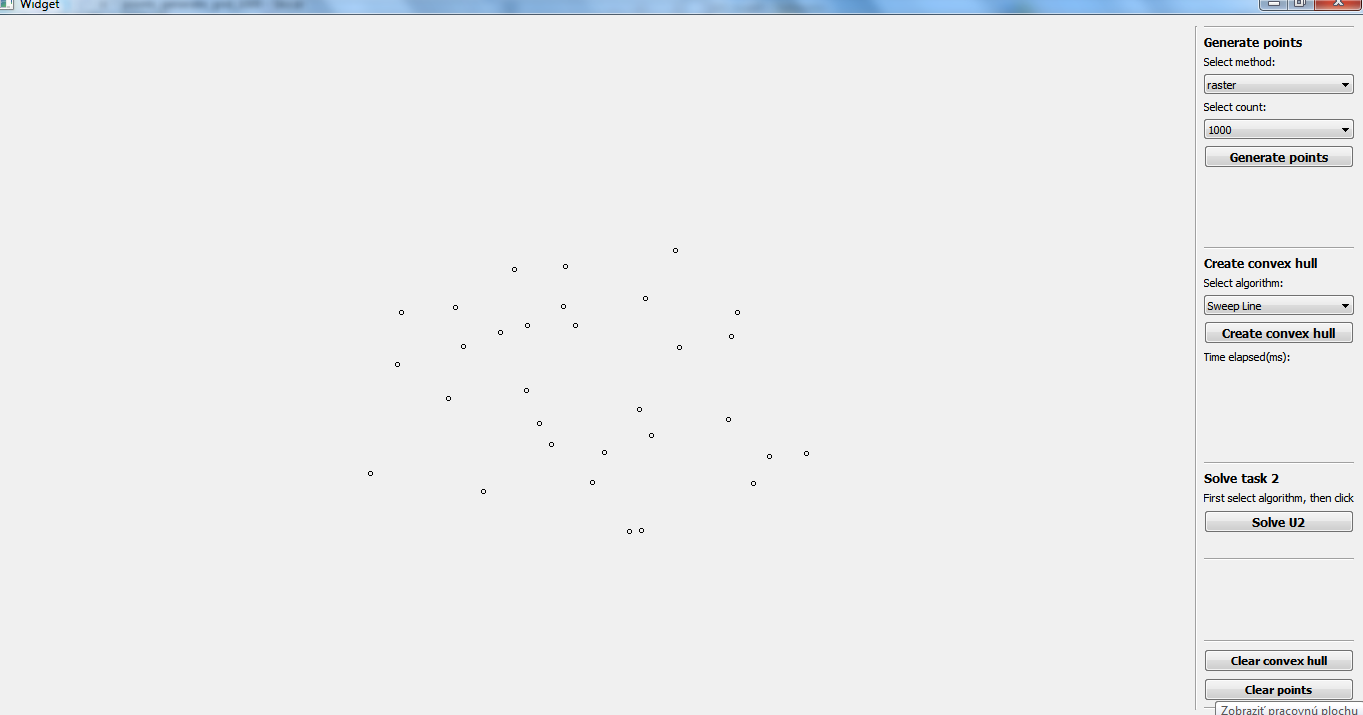
\includegraphics[width=10cm]{./img/points_manual.png}
   \captionof{figure}{Manuálne zadané body a vygenerová konvexná obálka}
\end{center}


\subsection{Automaticky generovaná množina bodov}
Množina vznikne automatickým vygenerovaním po zadaní požadovaného počtu generovaných bodov. Rozsah generovaných bodov je  n $\in$ $\langle$ 1000, 1000 000 $\rangle$ . Tvary generovaných bodov sú raster, kruh, náhodne generované body.

\begin{center}
   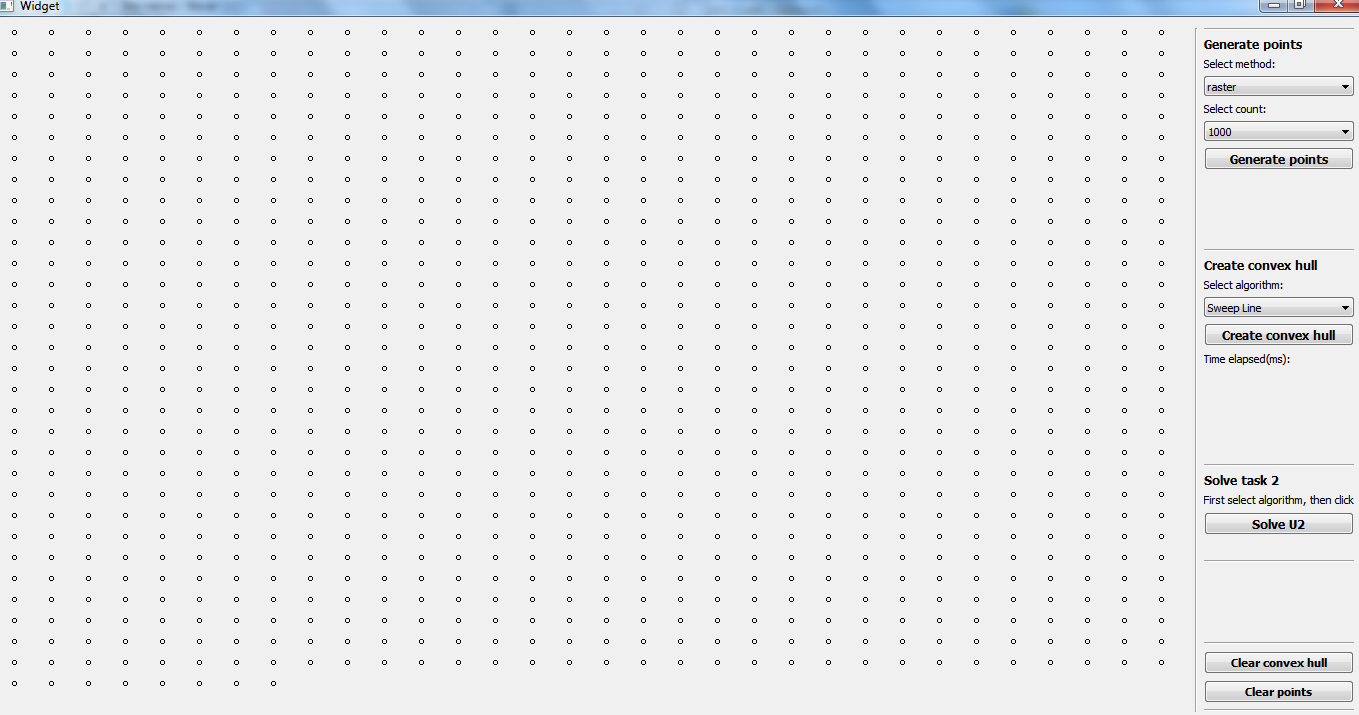
\includegraphics[width=10cm]{./img/points_generate_grid_1000.png}
   \captionof{figure}{Automaticky generovaných 1000 bodov v tvare rastru.}
\end{center}

\begin{center}
   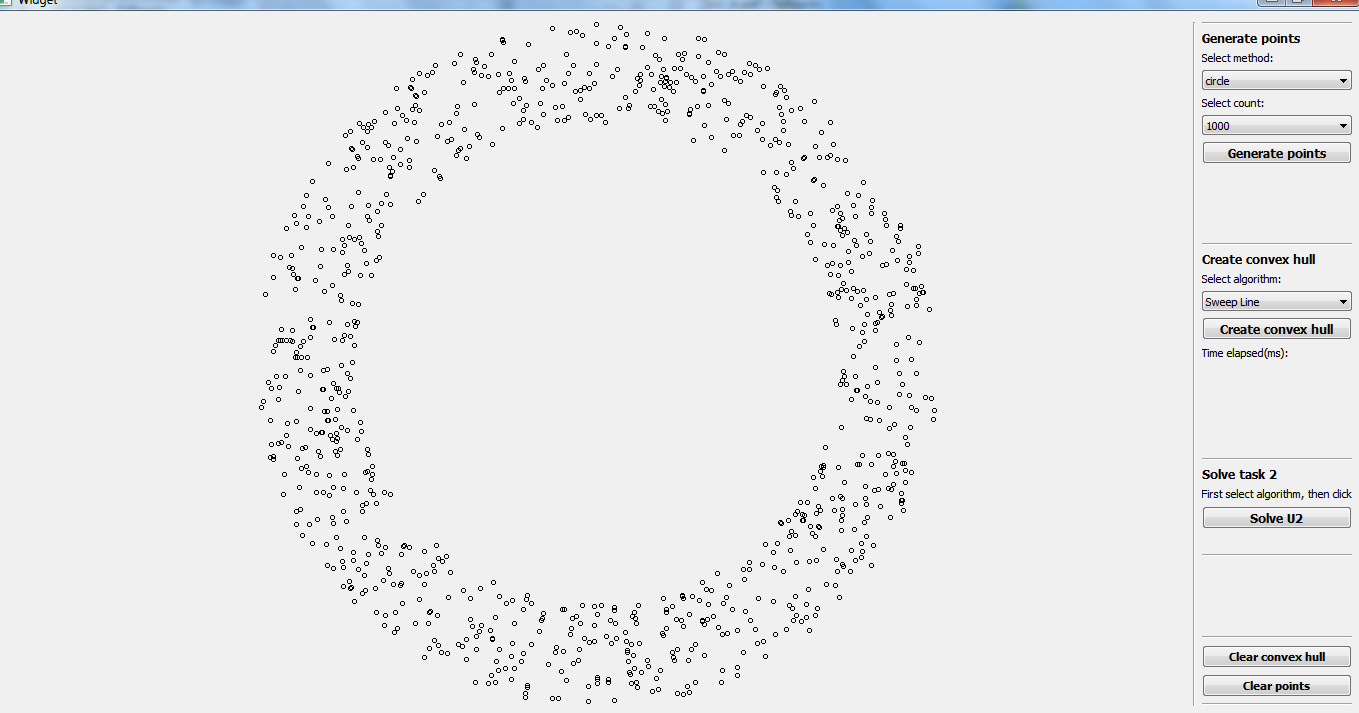
\includegraphics[width=10cm]{./img/points_generate_circle_1000.png}
   \captionof{figure}{Automaticky generovaných 1000 bodov v tvare kruhu.}
\end{center}

\begin{center}
   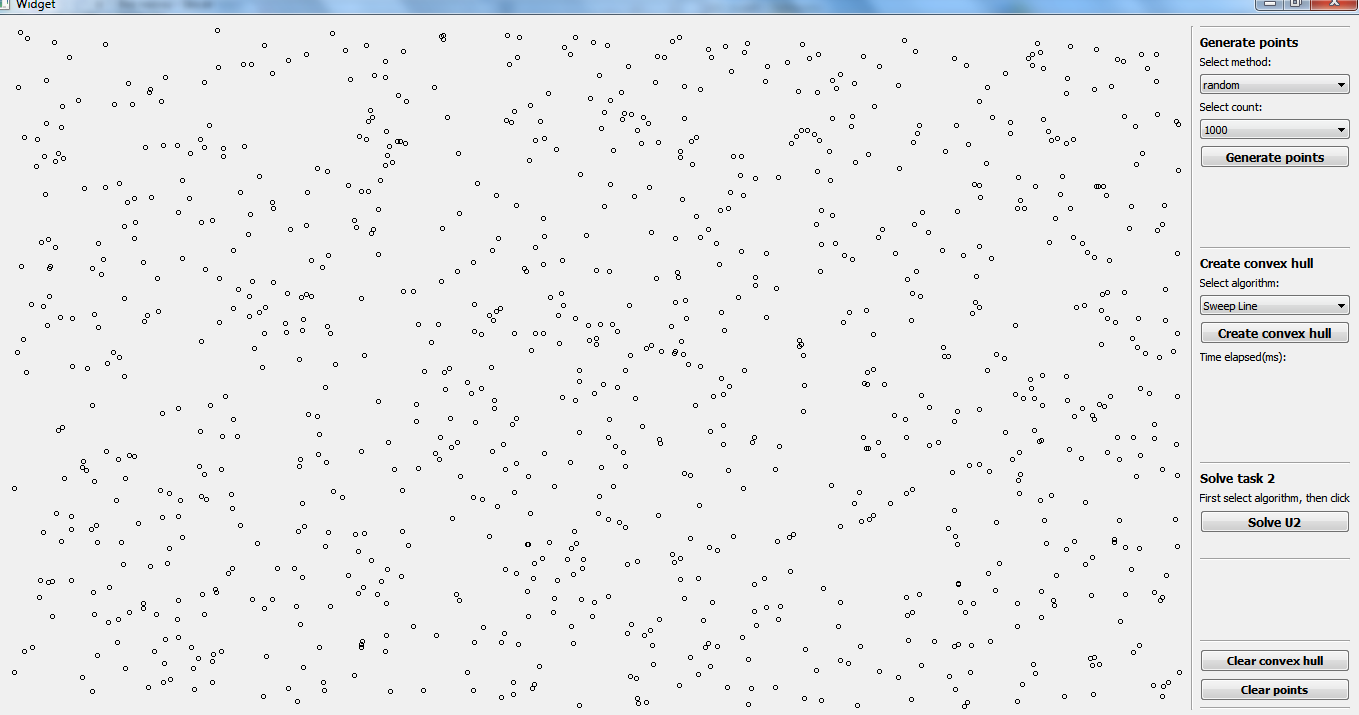
\includegraphics[width=10cm]{./img/points_generate_random_1000.png}
   \captionof{figure}{Automaticky generovaných 1000 bodov v náhodnom tvare.}
\end{center}

%------------------------------------------------------------------------
\clearpage 
\section{Ukážka vytvorenej aplikácie}

Grafické rozhranie aplikácie, vo svojej pravej časti, obsahuje možnosť generovania počtu bodov v užívateľom zvolenom tvare, vytvorenie konvexnej obálky pomocou zvoleného algoritmu. Pod tlačítkom \textit{Create convex hull} sa nachádza label v ktorom sa zobrazí doba trvania vygenerovania konvexnej obálky. Ďalej grafické rozhranie obsahuje tlačítko  \textit{Solve U2}. Po jeho stlačení sa zvoleným algoritmom prevedie generovanie konvexnej obálky automaticky. Toto generovanie prebieha automaticky 10x pre každý typ rozmiestnenia bodov ( raster, kruh, náhodné rozmiestnenie bodov) a počet bodov n $\in$ $\langle$ 1000, 5000, 10 000, 25 000, 50 000, 75 000, 100 000, 250 000, 500 000, 750 000, 1000 000 $\rangle$ . Pre každé generovanie konvexnej obálky je počítaná doba behu, ktorá sa spolu s počtom a typom generovaných bodov, typom algoritmu a poradím opakovania je ukladaná do textového súboru. Tento textový súbor je následne spracovaný v programe R Studio. Výsledné vytvorené grafy s porovnaním časovej náročnosti pri n počte vstupných bodov sú uvedené v kapitole \textit{Grafy a tabuľky}. 

\begin{center}
   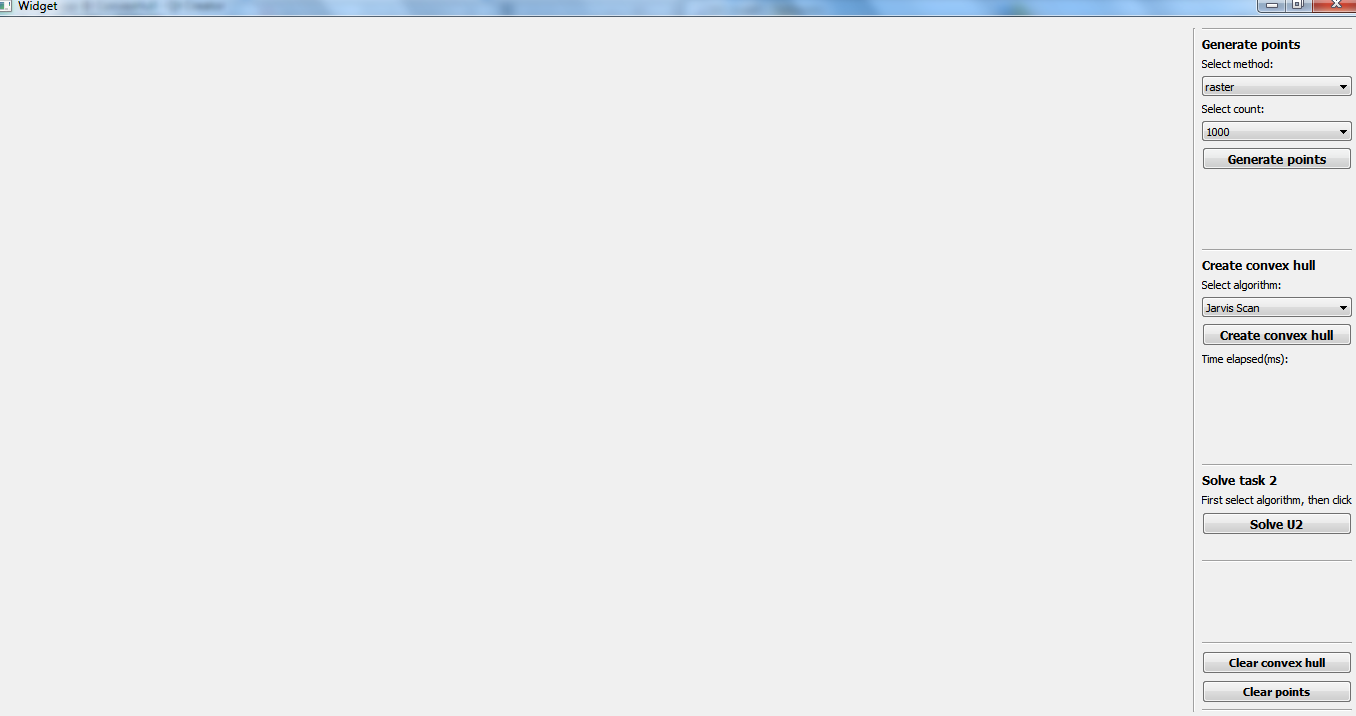
\includegraphics[width=10cm]{./img/ukazka_aplikacia1.png}
   \captionof{figure}{Ukážka grafického rozhrania aplikácie}
\end{center}


%-------------------------------------------------------------------------
\clearpage 
\section{Vykreslenie konvexnej obálky}
Po automatickom vygenerovaní bodov, prípadne ručnom naklikaní v Canvase , voľbe algoritmu konštrukcie konvexnej obálky a stlačení tlačidla \textit{Create convex hull} dostane užívateľ vygenerovanú konvexnú obálku. Pri genererovaní väčšieho počtu bodov ako $ n = 5000 $ sa v grafickom rozhraní vykreslí len prvých 5000 bodov, z dôvodu rýchlejšieho a jednoduchšieho vykreslovania. Konvexná obálka sa vygeneruje v plnom rozsahu.
 
\begin{center}
   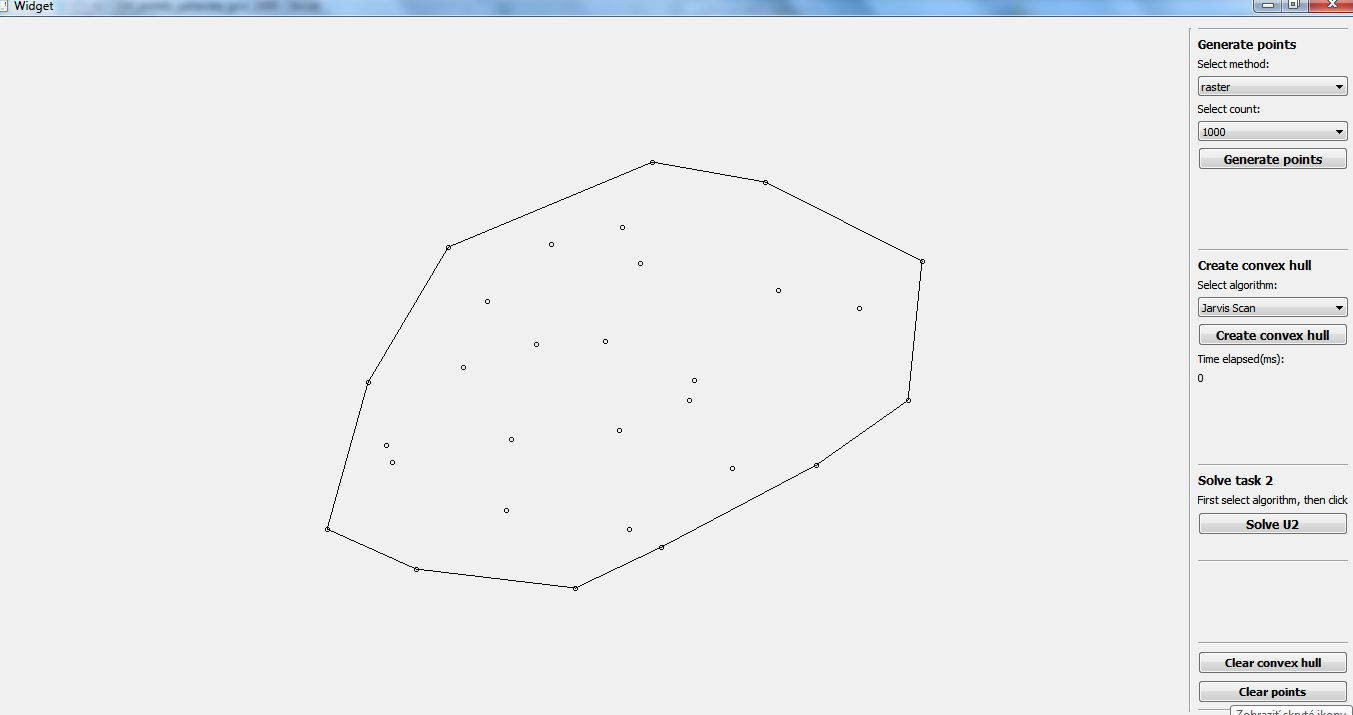
\includegraphics[width=10cm]{./img/CH_points_manual.png}
   \captionof{figure}{Manuálne zadané body a vygenerová konvexná obálka}
\end{center}

\begin{center}
   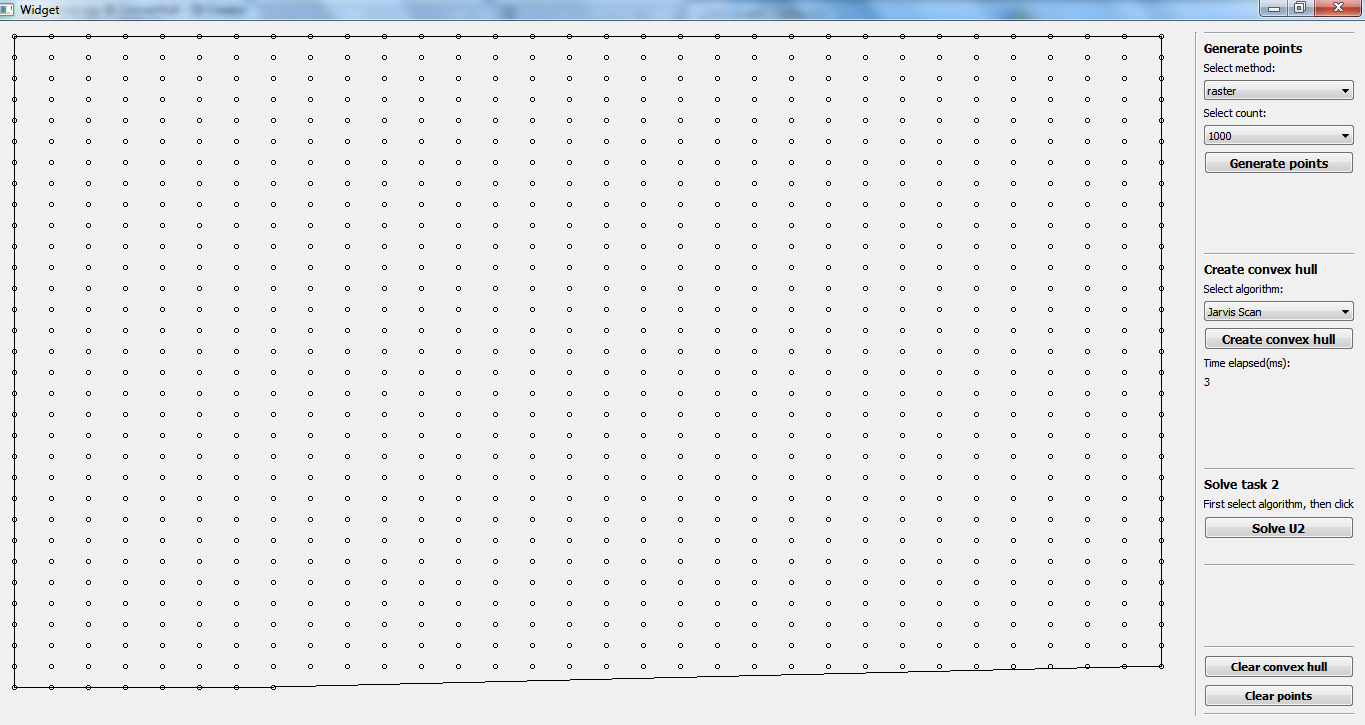
\includegraphics[width=10cm]{./img/CH_points_generate_grid_1000.png}
   \captionof{figure}{Automaticky generovaných 1000 bodov v tvare rastru, konvexná obálka bodov.}
\end{center}

\begin{center}
   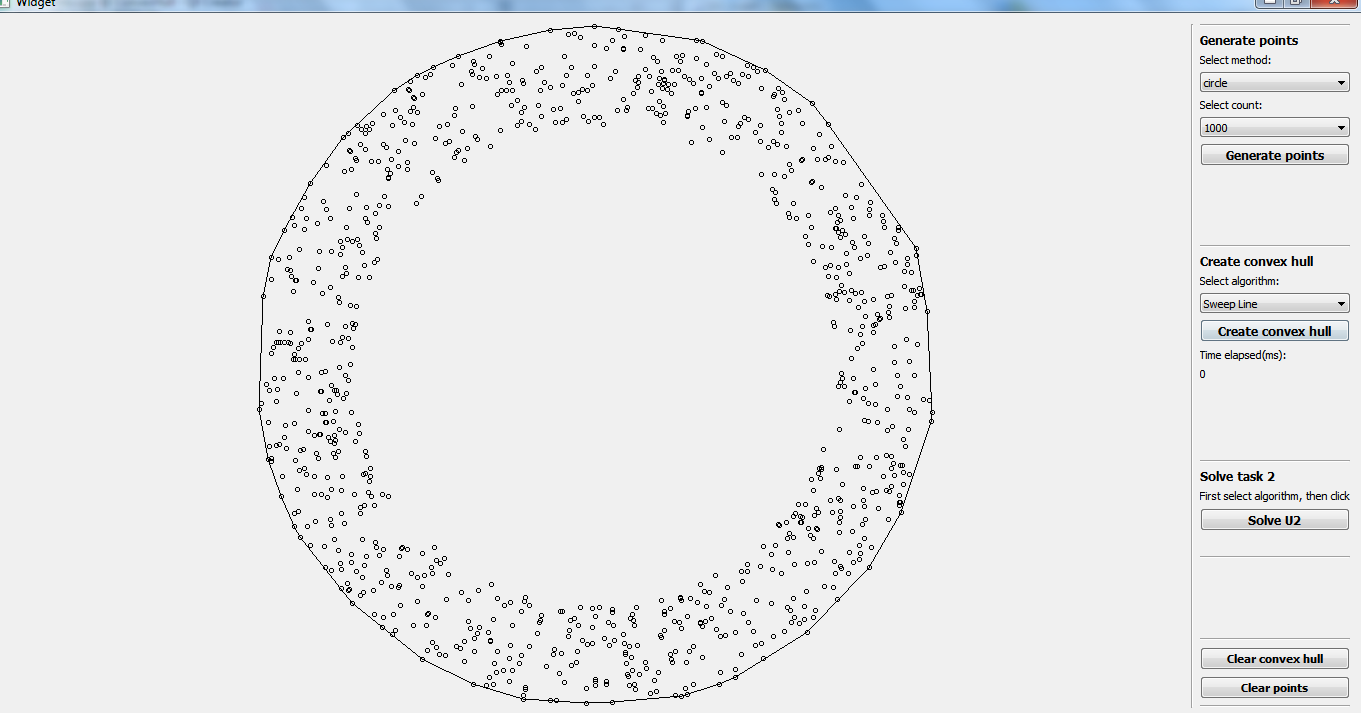
\includegraphics[width=10cm]{./img/CH_points_generate_circle_1000.png}
   \captionof{figure}{Automaticky generovaných 1000 bodov v tvare kruhu, konvexná obálka bodov.}
\end{center}

\begin{center}
   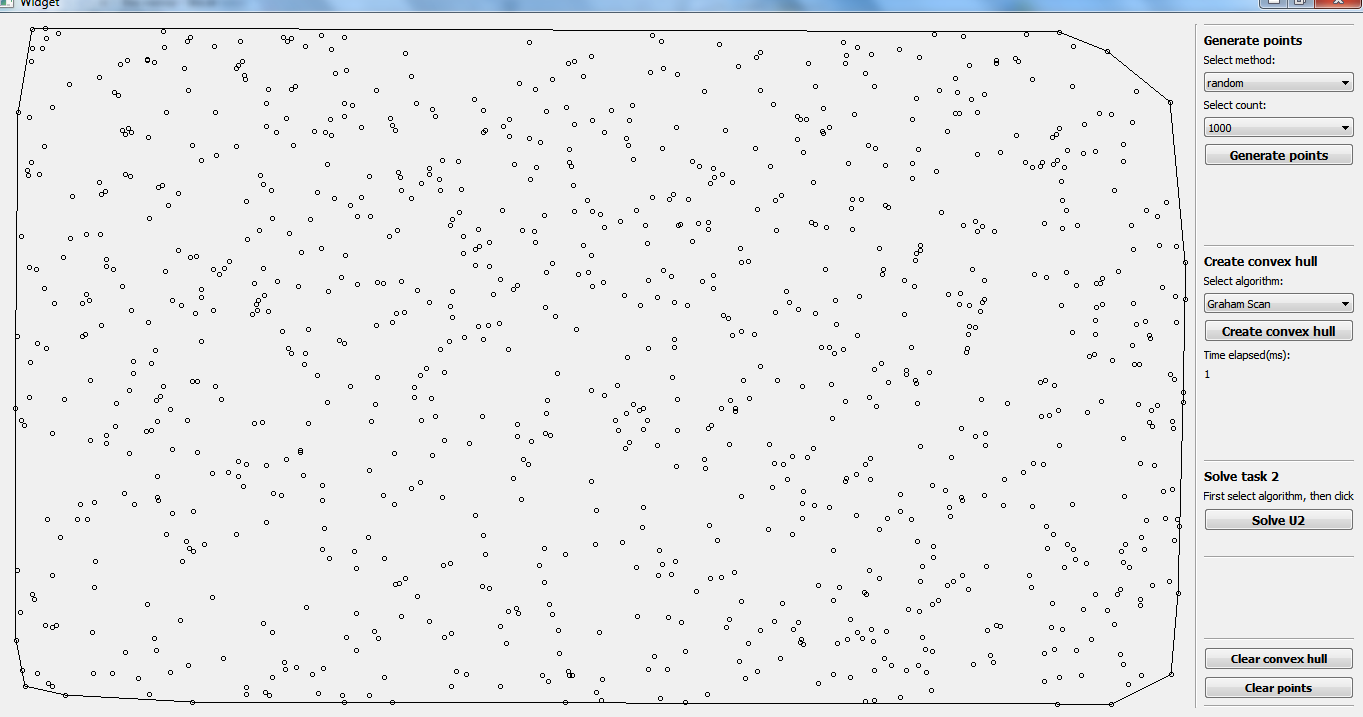
\includegraphics[width=10cm]{./img/CH_points_generate_random_1000.png}
   \captionof{figure}{Automaticky generovaných 1000 bodov v náhodnom tvare, konvexná obálka bodov.}
\end{center}
\clearpage
\begin{center}
   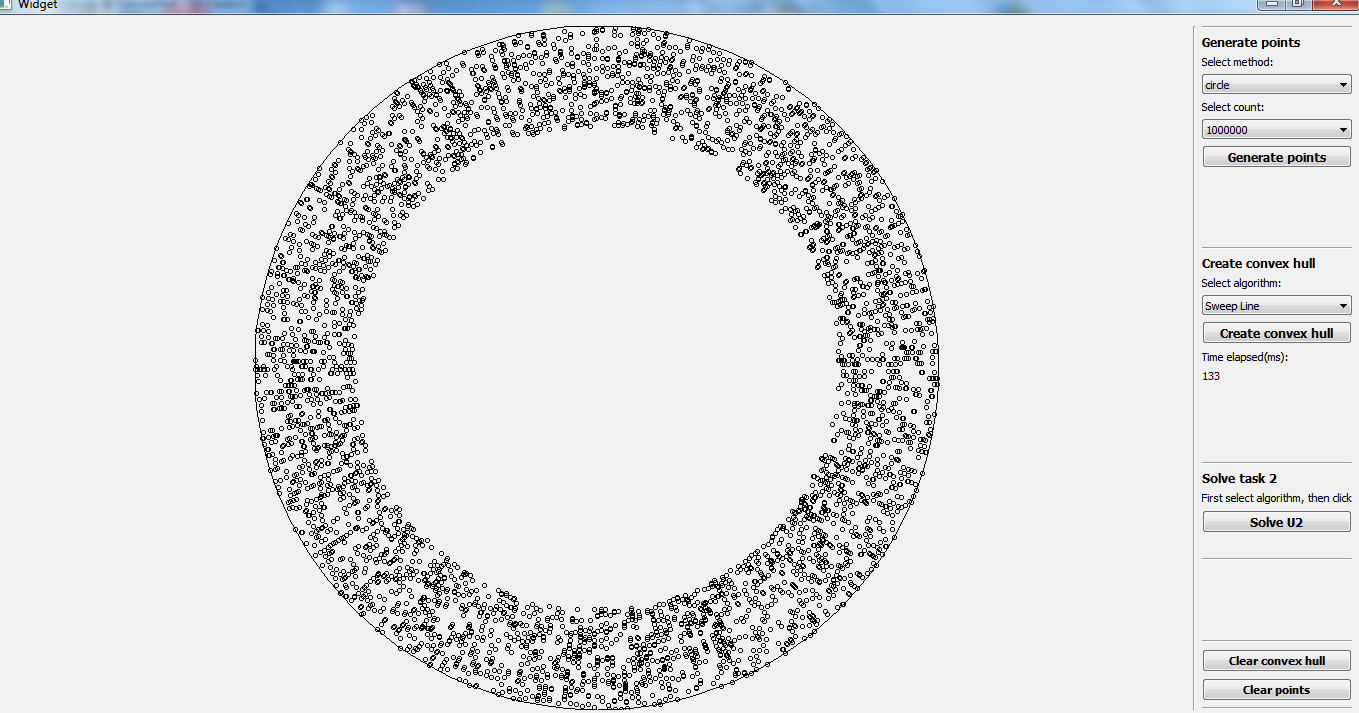
\includegraphics[width=10cm]{./img/milion_points.png}
   \captionof{figure}{Automaticky generovaných 1 000 000, konvexná obálka Sweep Line.}
\end{center}

%-------------------------------------------------------------------------
\clearpage 
\section{Grafy a tabuľky}



%-------------------------------------------------------------------------
\clearpage
\section{Dokumentácia}
\subsection{Trieda Algorithms}
Triedu Algorithms sme použili pre deklarovanie funkcií pre výpočtové algoritmy tvorby konvexnej obálky a pre deklaráciu ich pomocných metód.

\subsubsection{Členské premenné}

\begin{enumerate}
\item[] \underline{static QPoint pivot} 
\begin{itemize}
\item bod obsahujúci súradnice pivota
\end{itemize}
\item[] \underline{QPoint kolinear X point} 
\begin{itemize}
\item bod obsahujúci súradnice pomocného bodu, kolineárneho s osou X
\end{itemize}
\end{enumerate}

\subsubsection{Metódy}

\begin{enumerate}
\item[] \underline{getAngle2Vectors}
\begin{itemize}
\item Slúži k určeniu uhlu medzi dvoma priamkami. Jej návratovou hodnotou je double
\item na vstupe má : súradnice bodov $p_1, p_2, p_3, p_4$ určujúcich prvú a druhú priamku
\item výstupom je hodnota uhlu medzi priamkami 
\end{itemize}

\item[] \underline{getPointLinePosition}
\begin{itemize}
\item Slúži na určenie polohy bodu voči priamke. Jej návratovou hodnotou je integer.
\item na vstupe má : súradnice určovaného bodu q , súradnice bodov priamky $p_1$ $p_2$
\item na výstupe hodnoty :
\item[] -1 – bod sa nachádza na priamke
\item[] 0 – bod sa nachádza vpravo od priamky
\item[] 1 – bod sa nachádza vľavo od priamky
\end{itemize}

\item[] \underline{getPointLineDistance}
\begin{itemize}
\item je pomocnou metódou pre metódu positionPointPolygonWinding. Slúži na určenie polohy bodu voči priamke. Jej návratovou hodnotou je double.
\item na vstupe má : súradnice určovaného bodu q , súradnice bodov priamky $p_1$ $p_2$
\item na výstupe hodnotu vzdialenosti určovaného bodu od priamky.
\end{itemize}

\item[] \underline{Distance}
\begin{itemize}
\item Slúži na porovnanie vzdialenosti dvoch bodov. 
\item na vstupe má : súradnice bodov  $p_1$  a $p_2$
\item na výstupe hodnotu vzdialenosti medzi dvoma bodmi.
\end{itemize}

\item[] \underline{Angle}
\begin{itemize}
\item Slúži na porovnanie veľkosti dvoch uhlov. 
\item na vstupe má : súradnice bodov $p_1$ a $p_2$
\item na výstupe väčší uhol.
\end{itemize}

\item[] \underline{jarvisScan, qHull, grahamScan, sweepLine}
\begin{itemize}
\item Metódy slúžia k výpočtu konvexnej obálky podľa zvoleného výpočetného algoritmu. Vstupným typom je QPolygon
\item na vstupe je vektror bodov {std::vector}$<${QPoint}$>${points}
\item na výstupe je polygón obsahujúci množinu bodov a konvexnú obálku.
\end{itemize}

\item[] \underline{qh}
\begin{itemize}
\item Metódy slúžia k výpočtu konvexnej obálky podľa algoritmu Quick Hull. Je to pomocná metóda. Vstupným typom je void.
\item na vstupe je index počiatočného a koncového bodu deliacej priamky start, end
\item \hspace {1.5cm}  {std::vector}$<${QPoint}$>${points} vektor bodov okolo ktorých vytvárame konvexnú obálku
\item \hspace {1.5cm} QPolygon  convexHull ktorý obsahuje body konvexnej obálky
\item na výstupe je polygón obsahujúci konvexnú obálku.
\end{itemize}

\end{enumerate}

\subsection{Trieda Draw}
Trieda Draw slúži ku grafickému vykresleniu množiny modov a konvexnej obálky nad touto množinou.

\subsubsection{Členské premenné}
\begin{enumerate}

\item[] \underline {std::vector}$<${QPoint}$>${points}
\begin{itemize}
\item vektor bodov okolo ktorých vytvárame konvexnú obálku
\end{itemize}
\item[] \underline {QPolygon ch}
\begin{itemize}
\item polygón obsahujúci body konvexnej obálky
\end{itemize}
\end{enumerate}

\subsubsection{Metódy}
\begin{enumerate}
\item[] \underline{paintEvent}
\begin{itemize}
\item slúži k vykresleniu naklikaných a vygenerovaných bodov, vykresleniu konvexnej obálky. Návratovým typom je void.
\end{itemize}
\item[] \underline{void mousePressEvent}
\begin{itemize}
\item slúži k vykresleniu bodu  stlačením tlačidla myši, v okamihu stlačenia tlačidla na myši sa uložia súradnice bodu do vektoru points. Návratovým typom je void.
\end{itemize}
\item[] \underline{void clearCH}
\begin{itemize}
\item slúži k vymazaniu konvexnej obálky. Návratovým typom je void.
\end{itemize}
\item[] \underline{void clearPoints}
\begin{itemize}
\item slúži k vymazaniu množiny bodov. Návratovým typom je void.
\end{itemize}
\item[] \underline {std::vector}$<${QPoint}$>${getPoints}
\begin{itemize}
\item vektor, ktorý slúži k vráteniu množiny bodov points.
\end{itemize}
\item[] \underline {setCH}
\begin{itemize}
\item slúži na prevedenie konvexnej obálky do vykresľovacieho okna.
\end{itemize}
\item[] \underline {generatePoints}
\begin{itemize}
\item text.
\end{itemize}
\item[] \underline {generatePoints}
\begin{itemize}
\item slúži ku generovaniu množiny bodov. Na vstupe je zadaná metóda, počet bodov, šírka a výška.
\item na výstupe je vygenerovaná množina bodov podľa užívateľského zadania.
\end{itemize}
\item[] \underline {std::vector}$<${QPoint}$>${generatePointsU2}
\begin{itemize}
\item slúži ku generovaniu množiny bodov. Na vstupe je zadaná metóda, počet bodov, šírka a výška.
\item na výstupe je vygenerovaná množina bodov podľa užívateľského zadania. Generovanie konvexnej obálky prebehne automaticky 10x pre všetky typy tvaru generovanej množiny bodov a počty generovaných bodov v intervale od 1 000 do 1 000 000.
\end{itemize}
\end{enumerate}

\subsection{Tridy SortByX, SortByY}
Sú to triedy, ktoré obsahujú zoraďovacie kritériá. Pomocou týchto funkcií zoradíme súbor bodov podľa X alebo podľa Y súradnice.

\subsection{Trieda Widget}
Tieda Widget obashuje metódy ktoré sú odkazom na sloty umožňujúce vykonávať príkazy z grafického rozhrania aplikácie. Nemajú žiadne vstupné hodnoty, návratovým typom je void.

\subsubsection{Metódy}
\begin{enumerate}
\item[] \underline{on\_pushButton\_createCH\_clicked}
\begin{itemize}
\item tlačidlo \textbf{Create convex hull} po kliknutí naň sa vygeneruje konvexná obálka množiny bodov
\end{itemize}

\item[] \underline{on\_pushButton\_clearPoints\_clicked}
\begin{itemize}
\item tlačidlo \textbf{Clear points}  po kliknutí naň sa vymaže množina bodov
\end{itemize}

\item[] \underline{on\_pushButton\_clearCH\_clicked}
\begin{itemize}
\item tlačidlo \textbf{Clear convex hull}  po kliknutí naň sa vymaže konvexná obálka
\end{itemize}

\item[] \underline{on\_pushButton\_generatePoints\_clicked}
\begin{itemize}
\item tlačidlo \textbf{Generate points}  po kliknutí naň sa vygenerujú body v zvolenom tvare a počte
\end{itemize}

\item[] \underline{on\_pushButton\_solveU2\_clicked}
\begin{itemize}
\item tlačidlo \textbf{Solve U2}  po kliknutí naň sa vykoná automatické generovanie konvexnej obálky 10x pre každý typ rozmiestnenia bodov ( raster, kruh, náhodné rozmiestnenie bodov) a počet bodov n $\in$ $\langle$ 1000, 5000, 10 000, 25 000, 50 000, 75 000, 100 000, 250 000, 500 000, 750 000, 1000 000 $\rangle$ . Pre každé generovanie konvexnej obálky je počítaná doba behu, ktorá sa spolu s počtom a typom generovaných bodov, typom algoritmu a poradím opakovania je ukladaná do textového súboru
\end{itemize}

\end{enumerate}

%-------------------------------------------------------------------------
\clearpage
\section{Záver}

%-------------------------------------------------------------------------
\nocite{*}
%\printbibliography
\bibliography{literatura}{}
\bibliographystyle{plain}
%-------------------------------------------------------------------------
    
\end{document}             % Konec dokumentu.
